\documentclass[11pt,a4paper]{article}

\usepackage{times}
\usepackage{url}
\usepackage{graphicx}

\pagestyle{empty}

\textheight=25cm
\textwidth=15cm
\topmargin=-2cm
\oddsidemargin=0cm

\begin{document}

\begin{center}
  Ole Nielsen \\
  19 Melba Street
  Downer ACT 2602
  M: +61 401 966 202, \ \ \ E: Ole.Moller.Nielsen@gmail.com
\end{center}

\begin{center}
  \hrulefill \\
  {\bf CV} \\[-0.2cm]
  \hrulefill
\end{center}

\begin{center}
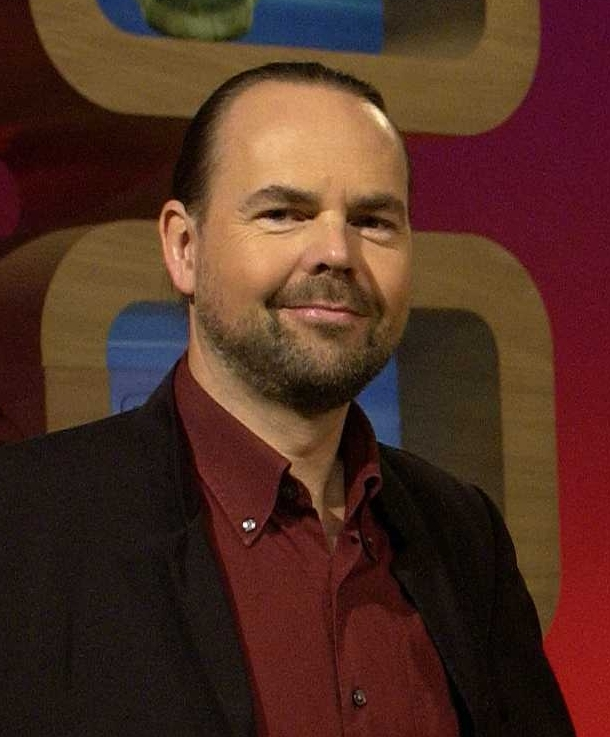
\includegraphics[width=50mm,keepaspectratio=true]{ole.jpg}
\end{center}

\begin{center}
  \hrulefill \\
  {\bf Mission} \\[-0.2cm]
  \hrulefill
\end{center}

\begin{center}
\emph{Focusing on issues that matter.}\\
\emph{Working together to achieve greatness.}\\
\emph{Embracing and driving change.}
\end{center}



\begin{center}
  \hrulefill \\
  {\bf Career History} \\[-0.2cm]
  \hrulefill
\end{center}

\begin{itemize}
\item {\em Feb 2017 -- Present}: Deputy Chief Digital Officer and Director of Digital Transformation, Chief Minister, Treasury and Economic Development Directorate, ACT Government.
      Supporting directorates to identify and implement digital transformation initiatives, empowering digital champions, challenging the status-quo through disruption and providing thought leadership to the ACT. Driving the implementation and uptake of the ACT Data Management Practice and iConnect. Formed the ACT Digital Champions which is a cross directorate community of practice concerned with hands-on digital transformation. 
\item {\em Apr 2014 -- Feb 2017}: Director of Scientific Computing and Systems Engineering, Geoscience Australia.
      Strategic leadership of software engineering, computational science and agile development.
      In particular, developed Digital Science Strategy for the agency and created team implementing automated continuous delivery to cloud which
      was a radically new approach.
      Identified the importance of the National Innovation and Science Agenda and the Digital Transformation Office. Became the Digital Transformation Coordinator for Geoscience Australia. Managed a budget of around five million dollars.
      Delivered 20+ IT projects every year.
\item {\em Mar 2013 -- Apr 2014}: Software Development Manager, Geoscience Australia.
      Oversight of software development, management of 40 staff, responsible for software quality and knowledge management. Started an Open Source agenda for the agency using GitHub which later grew to over 200 collaborative projects.
\item {\em Mar 2010 -- Mar 2013}: Numerical Modeller, Australia-Indonesia Facility for Disaster Reduction, AusAID, Indonesia.
      Oversight of software engineering and computational infrastructure supporting the Indonesian government disaster management agency in better planning and decision making. Lead developer of the InaSAFE impact modelling tool and real time earthquake impact prototype. Also technical oversight of initiatives including volcanic ash modelling project (Python FALL3D), seismology tools at BMKG (Bureau of Meteorology, Climatology and Geophysics) and Crowdsourcing of critical infrastructure using OpenStreetMap.
\item {\em Mar 2003 -- Mar 2010}: Senior Computational Scientist, Geoscience Australia.
      Research, development and application of natural hazard models. In particular, leading the development of the ANUGA hydrodynamic modelling tooland its application in tsunami impact modelling. Worked with states and territories to improve evacuation plans based on evidence from our models. Released ANUGA in 2006 as the first Open Source project from Geoscience Australia.
\item {\em Sep 2003 -- Dec 2003}: Visiting Professor,
      Department of Mathematics,
      Suranaree University of Technology, Nakhorn Ratchasima, Thailand. Teaching PhD course in
      High Performance Computing.
\item {\em Nov 1998 -- Feb 2003}: Research Fellow,
      School of Mathematical Sciences, Australian National University.
      Research in enterprise datamining, predictive modelling, machine learning and bioinformatics. Worked with CSIRO on data linkage and analytics of medical and pharmaceutical data to identify patterns in diagnosis and treatments. Developed and release the Open Source project Pypar which allows the Python programming language to use High Performance Computing platforms running Message Passing Interface (MPI).
\item {\em Mar 1998 -- Oct 1998}: Scientific Computing Consultant \\
      UNI$\bullet$C, Danish Computing Centre for Research and Education.\\
      Design and development of parallel image analysis algorithm for identification of anomalies in crops.
\end{itemize}

%\pagebreak
\begin{center}
  \hrulefill \\
  {\bf Education} \\[-0.2cm]
  \hrulefill
\end{center}

\begin{itemize}
\item Doctor of Philosophy (May 1998) \\
{\bf Technical University of Denmark} \\
Department of Mathematical Modelling  \\
Thesis: ``Wavelets in Scientific Computing''\\
%Available at {\tt http://datamining.anu.edu.au/\~{}ole} \\
%Grade Point Average: 11.0/13    %All 11's + one A

\item  Master of Science (November 1993) \\
{\bf Roskilde University, Denmark} \\
Department of Computer Science \\
Thesis: ``DISCO -- DIScrete and COntinuous simulation''\\
%Grade Point Average: 11.4/13  %(10.5 + 12 + 11 + 12)/4

\item  Batchelor of Science (June 1990) \\
{\bf Roskilde University, Denmark} \\
Department of Mathematics \\
%Grade Point Average: 11.5/13  %(10+13)/2
\end{itemize}

\pagebreak
\begin{center}
  \hrulefill \\
  {\bf Quotes From Colleagues} \\[-0.2cm]
  \hrulefill
\end{center}

\begin{itemize}
\item In Ole the ACT has found a rare talent: He deeply understands the mechanisms and potential for data systems and platforms but is also relentless in his approach to bring this back to the user and how the application of good data management can have a real impact on the very human interactions which drive service excellence. While this in itself may seem unremarkable Ole is able to combine his approach with a genuine appreciation for the challenges of service and cultural transformation at the Directorate and Government level which, with his open and authentic style, has made him a great advocate for change across complex organisational boundaries.
One of the few individuals capable of translating grand digital strategy to tangible business benefits, I have found Ole to be an excellent partner in our digital transformation and his influence is readily apparent in the cross-government solutions he has helped us to design and deliver.
\emph{John Bowdery, Director of Innovation and Customer Experience, Transport Canberra and City Services, ACT Government, 2017}

\item Ole has been a driver of digital innovation and collaboration across the ACT Government in his role as Deputy CDO. His open approach to engagement, depth of experience, and passion for digital transformation and its importance in driving modern government service delivery is an asset for the Territory. Ole has assisted education drive its digital transformation over the last year, especially with his assistance as a representative on the Schools Education Advisory Committee that provided expert advice to the Minister of Education on the best way to shape the device election commitment to ensure success in schools. Ole represented the office of the CDO effectively in this role and was a strong advocate and supporter of the implementation of innovative cloud services to progress this important reform.
\emph{Mark Huxley, Director Digital Strategy, Services and Transformation ACT Education Directorate, 2017}

\item Ole is an enlightened and very competent leader of digital change in the ACT Government. He has advanced the position of the CDO office through initiatives such as Digital Champions and Geospatial Working Groups. These forums have sparked more whole of Government innovation and collaboration than I've ever seen before. Ole's experience, vision and ability to communicate the innovation message to Government have inspired my team and I to participate in these forums and enable change. Ole keeps his finger on the pulse of technology developments and he has an immediate grasp of how it applies to delivering government services. His continued advice is key to the implementation of the Digital Strategy delivered by the Office of the CDO.
\emph{Jonathan Owen, Chief Information Security Officer, Shared Services, ACT Government, 2017}

\item For someone who’s tasked with driving digital transformation in government, to do more listening than talking, is refreshing. Ole is able to provide useful insights and examples from his own experience to assist in understanding business problems or developing business solutions. And his focus on people and not tech is a real strength in this area.
\emph{Dave Peffer, Deputy Director-General at Access Canberra, ACT Government, 2017}

\item I recently attended two government conferences and my favourite presenter was Ole Nielsen. His special blend of technical expertise as a software engineer in Denmark, his federal government experience and sound understanding of the technical challenges we face in the ACT Government made for two amusing and credible performances. Ole’s international experience blended with his great sense of humour made for two entertaining sessions and I wasn’t alone in saying his performance was a crowd favourite. I would highly recommended Ole as a guest speaker or for any senior role within government. Ole is well respected in the ACT Government digital community and has a great personality to deal with. I have been lucky enough to work closely with Ole this past year as a colleague trying drive digital innovation in the ACT. He has been a welcome addition to the digital office and I look forward to continue to have Ole provide his technical expertise to my teams over the coming months.
\emph{Kevin Bell, Deputy Director, Service Planning and Design, Access Canberra, ACT Government, 2017}

\item Ole always creates an inclusive and forward thinking atmosphere, releasing others from the belief that historic ways of working being the only way. Ole is able to take collective strategic ideas, combining them into an action plan that creates traction and momentum with participants, a critically important attribute to have in the digital world.
\emph{Garry Taylor, CIO, Community Services, ACT Government, 2017}

\item Ole has consistently demonstrated his commitment to the principles of digital work practices through the establishment of the digital champions network, representation of ACT Government in national digital fora, and through support and collaboration on digital programs of work across directorates. Ole is a great champion for the digital agenda and an effective motivator in building awareness and a desire for change in ACT Government.
Through Ole’s leverage of relationships across Canberra and his work in directorates he has demonstrated a deep appreciation of the challenges faced in unleashing hidden digital talent within government and how to innovate successfully within the constraints of a publicly funded environment. 
I have enjoyed working with Ole and have benefited greatly from his professional support and encouragement.
\emph{Cecilia Ridgley, Senior Manager, Strategic Innovation, Strategic Business, Shared Services, ACT Government, 2017}
  
  \item Ole has been at the forefront of software development at GA since his arrival in 2003, influencing not only those projects that he worked on directly but others such as the EQRM, a project that has benefited from Ole’s ideas around pair programming, unit testing, version control, issue tracking, documentation, and open-source. He is one of few at GA that can genuinely command respect as a scientist, a software developer and a manager.  He has a contagious level of enthusiasm and a willingness to find agency wide solutions that increase staff productivity in the science divisions. Ole is an inspiration to those of us that have worked with him. I am stronger at my job courtesy of time spent with Ole.
  \emph{Dr David Robinson (david.robinson@ga.gov.au), Geoscience Australia, 2014}
  \item Ole’s ideas in 2005 were right at the forefront of best practice and innovation in software development. That he was able to implement those ideas to deliver the highly complex ANUGA software and apply that to assist decision makers understand tsunami inundation risk is a unique achievement. \emph{Gordon Cheyne, Geoscience Australia, 2014}.
  \item Ole is not only an expert at software development; he is equally skilled at working with people, and is remarkable in his ability to build and lead interdisciplinary teams of technical specialists to develop products. This combination of technical and management expertises made Ole the ideal candidate to be seconded for three years to Jakarta to assist in establishing the Australia Indonesia Facility for Disaster Reduction (AIFDR) as part of a GA-AusAID portnership. Ole is extremely well respected by Indonesian colleagues in the technical/science community as well as in the emergecncy management stakeholder community. \emph{Dr John Schneider, Geoscience Australia, 2014}
  \item I use three software packages (PyPar, ANUGA and InaSAFE) that Ole has lead the development of as a core component of my day-to-day work. I use them because they are well-tested, robust open source software packages that are scientifically rigorous and adapted to solve the key science questions I face. I have worked with Ole since 2007 and find his drive and enthusiasm for applying state-of-the-art computational methods to complex scientific problems inspirational. \emph{Jonathan Griffin, Geoscience Australia, 2014}
  \item “Truly outstanding” is the best way to sum up the leadership that Ole has shown in the use of high performance computing and professional software engineering to support a wide range of applications within Geoscience Australia. \emph{GA AGM award 2008}.
  \item Ole’s discipline and demand for high quality software engineering has allowed the tsunami risk modelling team to undertake challenging cutting-edge projects for a number of clients with confidence that our tools can meet varied requirements. \emph{Dr Jane Sexton, Geoscience Australia, 2008}.
  \item Ole almost single handedly championed the idea of GA obtaining a Beuwolf cluster computer, by first developing a small test bed, gathering together a band of users and then being deeply involved in the subsequent business plan, tender, purchase and testing of the new GA system. \emph{Prof Stephen Roberts, ANU Dept Mathematics, 2006}.
  \item Ole published pypar at the time I was looking for a simple and high level library for communicating arrays from Python using MPI.  pypar was well written, easy to use, and open source.  This allowed me to easily parallelize my PhD code in 2004.
    \emph{Prabhu Ramachandran, Associate Professor, IIT Bombay}.
  \item Ole keynoted at the SciPy India 2012 conference that I helped organize and co-chaired.  Ole is one of the few enlightened researchers who understands the importance of following good software development practices in the context of scientific computing.  His experience and expertise in the application of these ideas to practical, scientific computational tools is clear to all who speak to him.  It was refreshing to see Ole's passion for open source software and his efforts to help society through scientific computing via the development of tools to help simulate the impact of tsunamis and floods.
    \emph{Prabhu Ramachandran, Associate Professor, IIT Bombay.} 
  \item It is always great to work with Ole on a project. He brings to the table impressive software engineering skills (I learnt to use unit testing under his influence), impressive scientific and mathematical skills (he incorporated a number of clever ideas into our tsunami simulation code, anuga) and finally and perhaps most importantly great people skills, always motivating and bringing together people with different skills (and personalities) to successfully complete sophisticated projects (the anuga project, the inasafe project).
    \emph{Prof Stephen Roberts, ANU Dept Mathematics, 2014}.
\item In June 2016 Dr Nielsen and I organised a ground breaking, three day, computational sciences workshop at Geosciences Australia. With limited support and an even more limited budget we leveraged AMSI’s membership and Ole’s contacts to deliver 20+ enthusiastic speakers and around 40 attendees. Ole’s leadership, both at GA and with the wider computational sciences community, was critical. The theme was bringing the mathematical sciences research community face to face with high level end users in the public agencies with a view to collaboration. Participants came from GA, NCI, BoM, ABS, CSIRO IMT and data 61, DSTGroup, ANU, QUT, UQ and AMSI Intern. In my opinion the workshop was an immediate success and its longer term success will be judged by the willingness of the participants to continue to engage.
  \emph{Professor Geoff Prince, Director, Australian Mathematical Sciences Institute}.
\item In my work as an earthquake and tsunami scientist I've seen Ole Nielsen progress over the past 13 years from a programming/numerical modeling role to a senior position as leader of scientific computing at GA. Ole has always deeply impressed me as a strategic thinker who is remarkably effective, not only in looking over the horizon to identify the important changes in computing that will advance our science, but in convincing those around him that changes can and must be made. Ole has brought about a profound change in the culture of scientific computing at GA, from one that feared change and was obsessed with security, to one that focusses on meeting the needs of its scientists. Ole's knowledge and depth of expertise in scientific computing is second to none, but it's really his formidable interpersonal skills that make him the kind of exceptional leader any institution will be lucky to have.
  \emph{Professor Phil Cummins, ANU, 2016}
%I've worked as an earthquake and tsunami scientist at GA and ANU for over 10 years, and during this time I've seen Ole Nielsen progress from a programming/numerical modeling role to a senior position as leader of scientific computing at GA. Ole has always deeply impressed me as a strategic thinker who is remarkably effective, not only in looking over the horizon to identify the important changes in computing that will advance our science, but in convincing those around him that changes can and must be made. As a scientist at GA I had long ago despaired at GA's inability to harness the power of "new" trends in scientific computing, things as basic as access to open source software and high performance computing. I sometimes scoffed at what I thought was Ole's naive vision that the strongly risk-averse management at GA would ever embrace these. But Ole proved me wrong at every turn. He has brought about a profound change in the culture of scientific computing at GA, from one that feared change and was obsessed with security, to one that focusses on meeting the needs of its scientists. Ole's knowledge and depth of expertise in scientific computing is second to none, but it's really his formidable interpersonal skills that make him the kind of exceptional leader NCI will be lucky to have.
  
\item  Ole is an inspirational leader who genuinely believes in his work. This genuinity means that people naturally congregate around Ole and his ideas, making him highly influential.

Ole’s extensive background in Scientific Computing and High Performance Computing combined with his ability to translate complex technical topics into simple language uniquely place him to convincingly communicate the value of Digital Science and High Performance Computing to anyone, from those neck deep in code to policy makers.

Ole’s leadership on developing GA’s first Digital Science Strategy was second to none. On a shoestring budget Ole managed to corral the enthusiasm and goodwill of those around him to delivery a strategy that people are proud to stand behind. Through establishing the Digital Science Agenda at GA, Ole has given digital scientists and Researchers a strong voice, and has kicked off an initiative that will drive GA towards becoming the modern science organisation we know it can be.

Ole understands that technology is about far more than state of the art infrastructure. Without a technologically imaginative society, we cannot even scratch the surface of the opportunities technology offers. Ole is one of very few people I have had the pleasure of working with who fully understands this.
\emph{Trent Kershaw, Geoscience Australia, 2016}

\item
  Ole has led a significant cultural and technical transformation of the scientific data and computing function and culture at Geoscience Australia.  Ole’s key strengths include: an ability to collaborate, partner and get buy-in from all stakeholders and staff; a strong understanding of contemporary ICT; and a focus on outcomes.  His leadership has driven the creation of a GA Digital Science Strategy that will drive the changes we need in the way we go about our science.
  \emph{Antony Stinziani, Geoscience Australia, 2016}

\item   I started working with Ole in 2006 at Geoscience Australia. In 2006 when I started at Geoscience Australia, Ole ran a Linux cluster that the minerals section utilised to run open source, innovative and time saving geophysical modelling inversions. Ole called his Linux clusters cyclone and tornado, because he was modelling weather. The collaboration between two very different science and management areas at GA lead to the largest modelling of Airborne Electromagnetic geophysical survey data in the world. This data would have taken years to compute if not for the Linux cluster. The cross pollination and multi-use of IT infrastructure hadn’t been seen on this scale in mineral geophysics ever before in Australia. Ole is an inspiring, inclusive and able leader and innovator in the field of digital transformation and information technology.\emph{Marina Costelloe, Geoscience Australia, 2017}.


\item
  When I started using ANUGA, a software whose development Ole led, I was positively surprised to find how well the software was programmed, documented and supported by Ole and his team members. Ole's help to succeed in using it for tsunami inundation modelling for Western Sumatra was invaluable and he was always more than helpful, diligent in his replies and insightful; he even assisted in adding an interface to use external data. He always showed an outstanding level of enthusiasm and capabilities to achieve a product useful for the entire community rather than a small group.
  \emph{Nils Goseberg, Senior Research Associate, Franzius-Institute for Hydraulic, Estuarine and Coastal Engineering, Leibniz Universität Hannover, 2016}

\item
  I first cold contacted Ole (by phone) in late 2006 regarding the release of the Government Funded Free and Open Source Software ANUGA, after finding his paper on line. I was delighted that he was openly approachable and eager to answer all of my questions. So much so that by early 2007 Ole had inspired me to discuss with him (and bring to fruition) the addition of functions to apply rainfall to the ANUGA model to allow riverine flood modelling. In 2008 Ole had offered to meet with Local Government to discuss the plausible concept of in-house flood modelling. This has extending to the concept of Flood Modelling Frameworks being hosted on the NCI, the first attempt being the ACT Flood Modelling Framework currenly hosted on the NCI.  
Through observing Ole's passion for creating a collaborative project I have also become a passionate contributor to the ANUGA project. Through his various roles since 2006 Ole has made it clear that he remains approachable and open to provide innovative suggestions to many computer issues (models, servers etc) that I strike from time to time. As such there continues an ongoing working relationship and warmly regarded friendship. Ole has an amazing skill in listening to various wide ranging professions (in my case engineering) and almost de-construct the complexities to enable him to provide invaluable advice and insight into how to solve computational issues.  
\emph{Rudy Van Drie, Consulting Engineer and Ex Local Government Flood Plain Management Engineer, 2014}

\item
I have known Ole since 2008 when I became involved in the use of ANUGA for flood modelling through a colleague. 2d flood modelling was in its infancy at that time and the commercial software available very expensive, so I needed an alternative.

I remember meeting with Ole to discuss the ability to model pipes under embankments. His enthusiasm was electric and within a day he had a concept for this idea working.

He saw back then what I see now with open source software, that everyone can contribute in their own small way to do some good.

Ole changed the way I work for the better and I am grateful for this.
  \emph{Dr Petar Milevski (pmilevski@gmail.com), Civil engineer urban drainage Wollongong city council, 2014}


\item I am professor at the Technical University of Denmark, and I was supervisor for Ole M. Nielsen’s PhD project on wavelets and their applications is scientific computing in the mid nineties.  Since then I have been following his career.
 
At that time, wavelets were making their way from a theoretical subject into the area of scientific computing, and the literature about their applications was a bit scattered.  Dr. Nielsen made a tremendous effort of “translating” the theoretical framework into a number of applications (e.g., image compression and solution of differential equations), and I admire his will and energy to continue his research even when he got stuck on either theory development or applications.  He wrote a remarkably pedagogical PhD theses which I used for a number of years to present this topic to students and colleagues.
 
At that time everyone wanted to write papers about how successful they were in using this new mathematical tool.  For that reason it was not always clear to distinguish the real success stories.  Dr. Nielsen showed a surprising maturity in not striving for making his results appear successful, but rather he took a critical perspective to pinpoint in which specific applications he saw wavelets having a real advantage.
 
Since then, his openness to new subjects and his critical eye has led to an interesting and successful career in scientific high-performance computing
\emph{Professor Per Christian Hansen, Section for Scientific Computing, Technical University of Denmark, 2016}

\end{itemize}


\begin{center}
  \hrulefill \\
  {\bf Selected achievements} \\[-0.2cm]
  \hrulefill
\end{center}

\begin{itemize}
\item Developed Digital Science Strategy for Geoscience Australia through deep consultation with scientists, executives and ICT staff in the agency as well as our partners CSIRO, BoM, DSTG and the NCI. This strategy outlines how science is changing as a result of the digital disruption that is currently happening and how Geoscience Australia therefore must also change. It describes the importance of getting the right skills to bear on our priorities, how we must adopt an agile way of working to remain relevant, the importance of a seamless technology platforms where applications can be ported as required, how we must change our processes to support innovation and that leadership of this must sit at the executive level. This strategy is shaping the agency as evidenced by the recent restructure of ICT to Digital Science and Information Branch in Geoscience Australia. 
  \item Built cohesive team of almost 40 software developers following centralisation of software development in Geoscience Australia and implemented agreed quality measures and development standards for the main development languages in use in the organisation. I lead the increased focus on Continuous Delivery, Open Source, Test Automation and Cloud Computing as well as day to day people management and conflict resolution.
  \item Lead the development of a novel and user friendly application for rapid and reproducible estimation of impact from natural disasters called InaSAFE which is available at \url{www.inasafe.org}.
  Version 1.0 was publicly and officially launched at the Asian Ministerial Conference on Disaster Risk Reduction in October 2012 and shown to the president of Indonesia as the centrepiece of Australian Indonesian cooperation in Disaster Management. InaSAFE is currently being provided to local and national disaster managers in Indonesia. The World Bank who is a partner in this project is building web applications based on InaSAFE for use world wide.
  InaSAFE won the Black Duck prize for most promising projects of 2012. % \url{http://www.blackducksoftware.com/news/releases/black-duck-announces-2012-open-source-rookies-year-winners}
  \item The ANUGA hydrodynamic modelling project which is a sophisticated open source software model written in Python and C, that has underpinned all tsunami inundation modelling in Australia. Under my leadership, this project lead to two AGM team awards: 2006 (Capability) and 2007 (Influence); was featured in 2009 in a special episode on the Australian TV program The New Inventors \emph{Dealing With Disasters} and attracted the Emergency Management Australia "Safer Communities Award" in 2005 and 2007 as well as the "Asia-Pacific Spatial Excellence Award" in 2007. ANUGA was developed as a strongly test driven project (now with almost 1,000 unit tests) and a comprehensive regression test suite of physical validation examples. ANUGA was released as Open Source in December 2006 (the first from GA) and has since then had over 16,000 downloads and is now used widely outside the organisation - e.g.\ for urban flood modelling: \url{http://en.wikipedia.org/wiki/ANUGA_Hydro}
  %\item A new modelling capability, ANUGA, that can simulate
  %impacts of tsunami, storm surge or flood disasters on the built environment.
  %This work was awarded the Emergency Management Australia "Safer Communities Award" in 2005 and 2007 as well as the
  %Asia-Pacific Spatial Excellence Award in 2007.
  %More information about the ANUGA project is available at \url{http://en.wikipedia.org/wiki/ANUGA_Hydro}
  \item A corporate high performance computing capability in my organisation.
  This involved building a prototype parallel Linux cluster, developing and presenting the business case to the
  senior management team, setting up a corporate wide special interest group, managing the installation process
  from tender to final acceptance testing.
  \item Influencing workplace to take up modern software development methodologies and practices that have improved the quality, speed and audit trail of corporate software.
  \item A binding for the Message Passing Interface (MPI) for the Python programming language.
  Pypar is open source, used widely in the scientific community (bio-informatics, health and datamining and modelling) and underpins projects such as ANUGA, python-FALL3D, URS-TSUNAMI and EQRM.
  Pypar is available at \url{http://code.google.com/p/pypar}
  \item The development of a WEB-enabled
  data exploration tool online analysis of large Health care databases
  at the Health Insurance Commission. This involved datamining and record linkage of about 80 million
  MBS claims and 50 million PBS claims and required the development of special purpose software to
  handle these volumes.
  %\item Designed and developed an open software library for data mining
  %of large relational databases using the scripting language Python
  %This library is successfully used for fast, interactive access to large
  %databases at the Australian National University (ANU) and
  %Commonwealth Science and Industrial Research Organisation (CSIRO).
  %\item Developed database of currently 0.5 million
  %GPS coordinates searchable by proximity to a given location
  %and by optional keywords. The search engine is fast
  %due to data base tables dynamically organised in a tree structure.
  %Wrote WEB front end for searching, retrieving and uploading GPS waypoints
  %using the GPS search engine.
  %\item Successfully implemented and applied a wavelet based algorithm
  %for surface fitting of high-dimensional data for use in predictive modelling.
  \item Developed vector-parallel fast wavelet transforms
  for the Fujitsu scientific software library.
  % at the Australian National University.
  The implementation was accompanied by a performance model that
  predicted both sequential and parallel actual performance.
  About 80 \% of peak performance on one processor was achieved,
  and the parallel efficiency was {\em independent} of the problem size
  as well as the number of processors.
  \item Developed an efficient algorithm for
  wavelet transforms of circulant matrices
  and various operations on them.
  Exploiting the particular structure of this problem
  reduced the storage requirements as well as the algorithmic complexity
  from {\em quadratic} to {\em linear} in the number of non-zeros.
  %\item Did the initial analysis, design, and architecture evaluations
  %towards the parallelisation of a medical image analysis algorithm.
  %\item Published an easy-to-understand wavelet tutorial
  %in IEEE Computer Applications in Power, Volume 12, Number 1, January 1999.
  %\item Have given technical and scientific presentations at
  %various institutions and conferences including
  %International Disaster Reduction Conference (Switzerland 2006);
  %UNESCAP High Level Technical meeting on Tsunami Disasters (Thailand 2005);
  %Australian Earth Quake Engineers annual meeting (GA 2006), Dynamic Earth Conference (ANU 2006),
  %Computational Techniques and Applications Conferences (CTAC 1999, 2006);
  %Modelling and Simulations (MODSIM 2005), Ninth Internal Python Conference (Californa 2001),
  %Australian Epidemiological Association (Sydney); NSW Health; IBM Yorktown heights (USA);
  %St Catherine's College, Oxford (UK); Umeaa University (Sweden);
  %UNI$\bullet$C (Denmark); and many more.
\end{itemize}


\begin{center}
  \hrulefill \\
  {\bf Selected publications} \\[-0.2cm]
  \hrulefill
\end{center}

\input{cv_publ.sub}



\end{document}

